\documentclass[
11pt, % The default document font size, options: 10pt, 11pt, 12pt
%codirector, % Uncomment to add a codirector to the title page
]{charter} 


% El títulos de la memoria, se usa en la carátula y se puede usar el cualquier lugar del documento con el comando \ttitle
\titulo{Sistema inteligente de optimización de compras de supermercado con pronóstico de precios y detección de ofertas engañosas} 

% Nombre del posgrado, se usa en la carátula y se puede usar el cualquier lugar del documento con el comando \degreename
%\posgrado{Carrera de Especialización en Sistemas Embebidos} 
%\posgrado{Carrera de Especialización en Internet de las Cosas} 
\posgrado{Carrera de Especialización en Inteligencia Artificial}
%\posgrado{Maestría en Sistemas Embebidos} 
%\posgrado{Maestría en Internet de las cosas}

% Tu nombre, se puede usar el cualquier lugar del documento con el comando \authorname
% IMPORTANTE: no omitir titulaciones ni tildación en los nombres, también se recomienda escribir los nombres completos (tal cual los tienen en su documento)
\autor{Ing. Nicolás Francisco Moguilner Reh}

% El nombre del director y co-director, se puede usar el cualquier lugar del documento con el comando \supname y \cosupname y \pertesupname y \pertecosupname
\director{Dr. Ing. Facundo Adrián Lucianna}
\pertenenciaDirector{FIUBA} 
\codirector{} % para que aparezca en la portada se debe descomentar la opción codirector en los parámetros de documentclass
\pertenenciaCoDirector{FIUBA}

% Nombre del cliente, quien va a aprobar los resultados del proyecto, se puede usar con el comando \clientename y \empclientename
\cliente{Dr. Ing. Facundo Adrián Lucianna}
\empresaCliente{FIUBA}
 
\fechaINICIO{19 de octubre de 2026}		%Fecha de inicio de la cursada de GdP \fechaInicioName
\fechaFINALPlan{14 de diciembre de 2026} 	%Fecha de final de cursada de GdP
\fechaFINALTrabajo{16 de agosto de 2027}	%Fecha de defensa pública del trabajo final


\begin{document}

\maketitle
\thispagestyle{empty}
\pagebreak


\thispagestyle{empty}
{\setlength{\parskip}{0pt}
\tableofcontents{}
}
\pagebreak


\section*{Registros de cambios}
\label{sec:registro}


\begin{table}[ht]
\label{tab:registro}
\centering
\begin{tabularx}{\linewidth}{@{}|c|X|c|@{}}
\hline
\rowcolor[HTML]{C0C0C0} 
Revisión & \multicolumn{1}{c|}{\cellcolor[HTML]{C0C0C0}Detalles de los cambios realizados} & Fecha      \\ \hline
0      & Creación del documento                                 &\fechaInicioName \\ \hline
1      & Se completa hasta el punto 5 inclusive                & 30 de octubre de 2026 \\ \hline
%2      & Se completa hasta el punto 9 inclusive
%		  Se puede agregar algo más \newline
%		  En distintas líneas \newline
%		  Así                                                    & {día} de {mes} de 202X \\ \hline
%3      & Se completa hasta el punto 12 inclusive                & {día} de {mes} de 202X \\ \hline
%4      & Se completa el plan	                                 & {día} de {mes} de 202X \\ \hline

% Si hay más correcciones pasada la versión 4 también se deben especificar acá

\end{tabularx}
\end{table}

\pagebreak



\section*{Acta de constitución del proyecto}
\label{sec:acta}

\begin{flushright}
Buenos Aires, \fechaInicioName
\end{flushright}

\vspace{2cm}

Por medio de la presente se acuerda con el \authorname\hspace{1px} que su Trabajo Final de la \degreename\hspace{1px} se titulará ``\ttitle'' y consistirá en el desarrollo y la evaluación de un prototipo de sistema basado en aprendizaje automático que, a partir de los datos abiertos de precios de supermercados de Argentina (SEPA), recomiende dónde, cuándo y con qué medio de pago realizar una compra para pagar lo mínimo, y que detecte ofertas engañosas. El trabajo tendrá un presupuesto preliminar estimado de 600 horas y sin costos directos previstos a priori, salvo eventuales gastos asociados a servicios en la nube, \textit{hosting}, \textit{marketplaces} u otros servicios de terceros, con fecha de inicio el \fechaInicioName\hspace{1px} y fecha de presentación pública el \fechaFinalName.

Se adjunta a esta acta la planificación inicial.

\vfill

% Esta parte se construye sola con la información que hayan cargado en el preámbulo del documento y no debe modificarla
\begin{table}[ht]
\centering
\begin{tabular}{ccc}
\begin{tabular}[c]{@{}c@{}}Dr. Ing. Ariel Lutenberg \\ Director posgrado FIUBA\end{tabular} & \hspace{2cm} & \begin{tabular}[c]{@{}c@{}}\clientename \\ \empclientename \end{tabular} \vspace{2.5cm} \\ 
\multicolumn{3}{c}{\begin{tabular}[c]{@{}c@{}} \supname \\ Director del Trabajo Final\end{tabular}} \vspace{2.5cm} \\
\end{tabular}
\end{table}




\section{1. Descripción técnica-conceptual del proyecto a realizar}
\label{sec:descripcion}

El presente trabajo es un emprendimiento personal del autor, desarrollado en el marco del Trabajo Final de la \degreename. No cuenta con financiamiento de programas públicos ni privados y no está sujeto a acuerdos de confidencialidad. Los datos principales son abiertos (licencia CC BY 4.0) y la propiedad intelectual de los entregables corresponde al autor.

\textbf{El problema.} Una persona tiene su lista de compras y quiere saber dónde, cuándo y con qué medio de pago le conviene comprarla. La decisión no es trivial: en Argentina los precios se remarcan cada pocas semanas; cada cadena, banco y billetera virtual ofrece descuentos con días, porcentajes, segmentos (por ejemplo, jubilados), exclusiones y topes distintos; un mismo producto puede encontrarse en otra marca o presentación; y en fechas como CyberMonday o Black Friday es habitual que un precio suba antes de la promoción para luego ``bajar''. Por ejemplo, en un ticket real de Coto (La Plata, 16/11/2024) una compra de \$\,33.372 abonada con un descuento anunciado del 15\,\% ``sin tope'' de Mercado Pago obtuvo una rebaja de \$\,1.173, es decir, un 3,5\,\% efectivo, debido a las exclusiones de productos.

\textbf{Estado del arte.} Desde 2016 las cadenas de supermercados más grandes están obligadas a informar a diario sus precios por sucursal al Sistema Electrónico de Publicidad de Precios Argentinos (SEPA). Actualmente se publican los precios de alrededor de 3.100 sucursales de 17 empresas en 24 jurisdicciones, con código de barras, precio por unidad de medida y hasta dos promociones por producto. El portal oficial solo conserva los últimos siete días. Sobre estos datos existen comparadores como preciazo, ratoneando, SEPAME y Yoper, que muestran el precio del día, pero no pronostican precios, no consideran el medio de pago del usuario, no detectan descuentos engañosos y no evalúan la conveniencia de un precio en el tiempo. En la Unión Europea, la Directiva Ómnibus establece que el precio de referencia de un descuento debe ser el mínimo de los 30 días previos, criterio que se toma como referencia para detectar ofertas engañosas. Entre los trabajos finales de la CEIA presentados hasta junio de 2026 no se encontraron trabajos que aborden precios de supermercado, ofertas engañosas ni medios de pago.

\textbf{La solución propuesta.} Se propone un sistema que, dada una lista de compras y el perfil de medios de pago del usuario, recomiende la sucursal, el día y el medio de pago que minimizan el costo esperado, y que alerte sobre ofertas engañosas. La propuesta de valor es un ahorro medible en pesos frente a la forma habitual de comprar (un mismo supermercado, el día de siempre y cualquier medio de pago). Además, a sugerencia de la coordinación académica, el usuario podrá consultar si un precio visto fuera de las cadenas principales (por ejemplo, en un almacén) es conveniente frente a los datos disponibles.

En la figura \ref{fig:diagBloquesProyecto} se presenta el diagrama en bloques del sistema. Se observa que las fuentes de datos alimentan un módulo de ingesta, cuya salida se unifica a nivel de producto y luego se utiliza en los modelos de pronóstico y de detección de ofertas engañosas, que a su vez alimentan al optimizador. Los bloques en gris con borde punteado corresponden a funcionalidades opcionales, fuera del alcance base, que se incorporarán solo si el cronograma lo permite (ver sección \ref{sec:alcance}).

\begin{figure}[htpb]
\centering
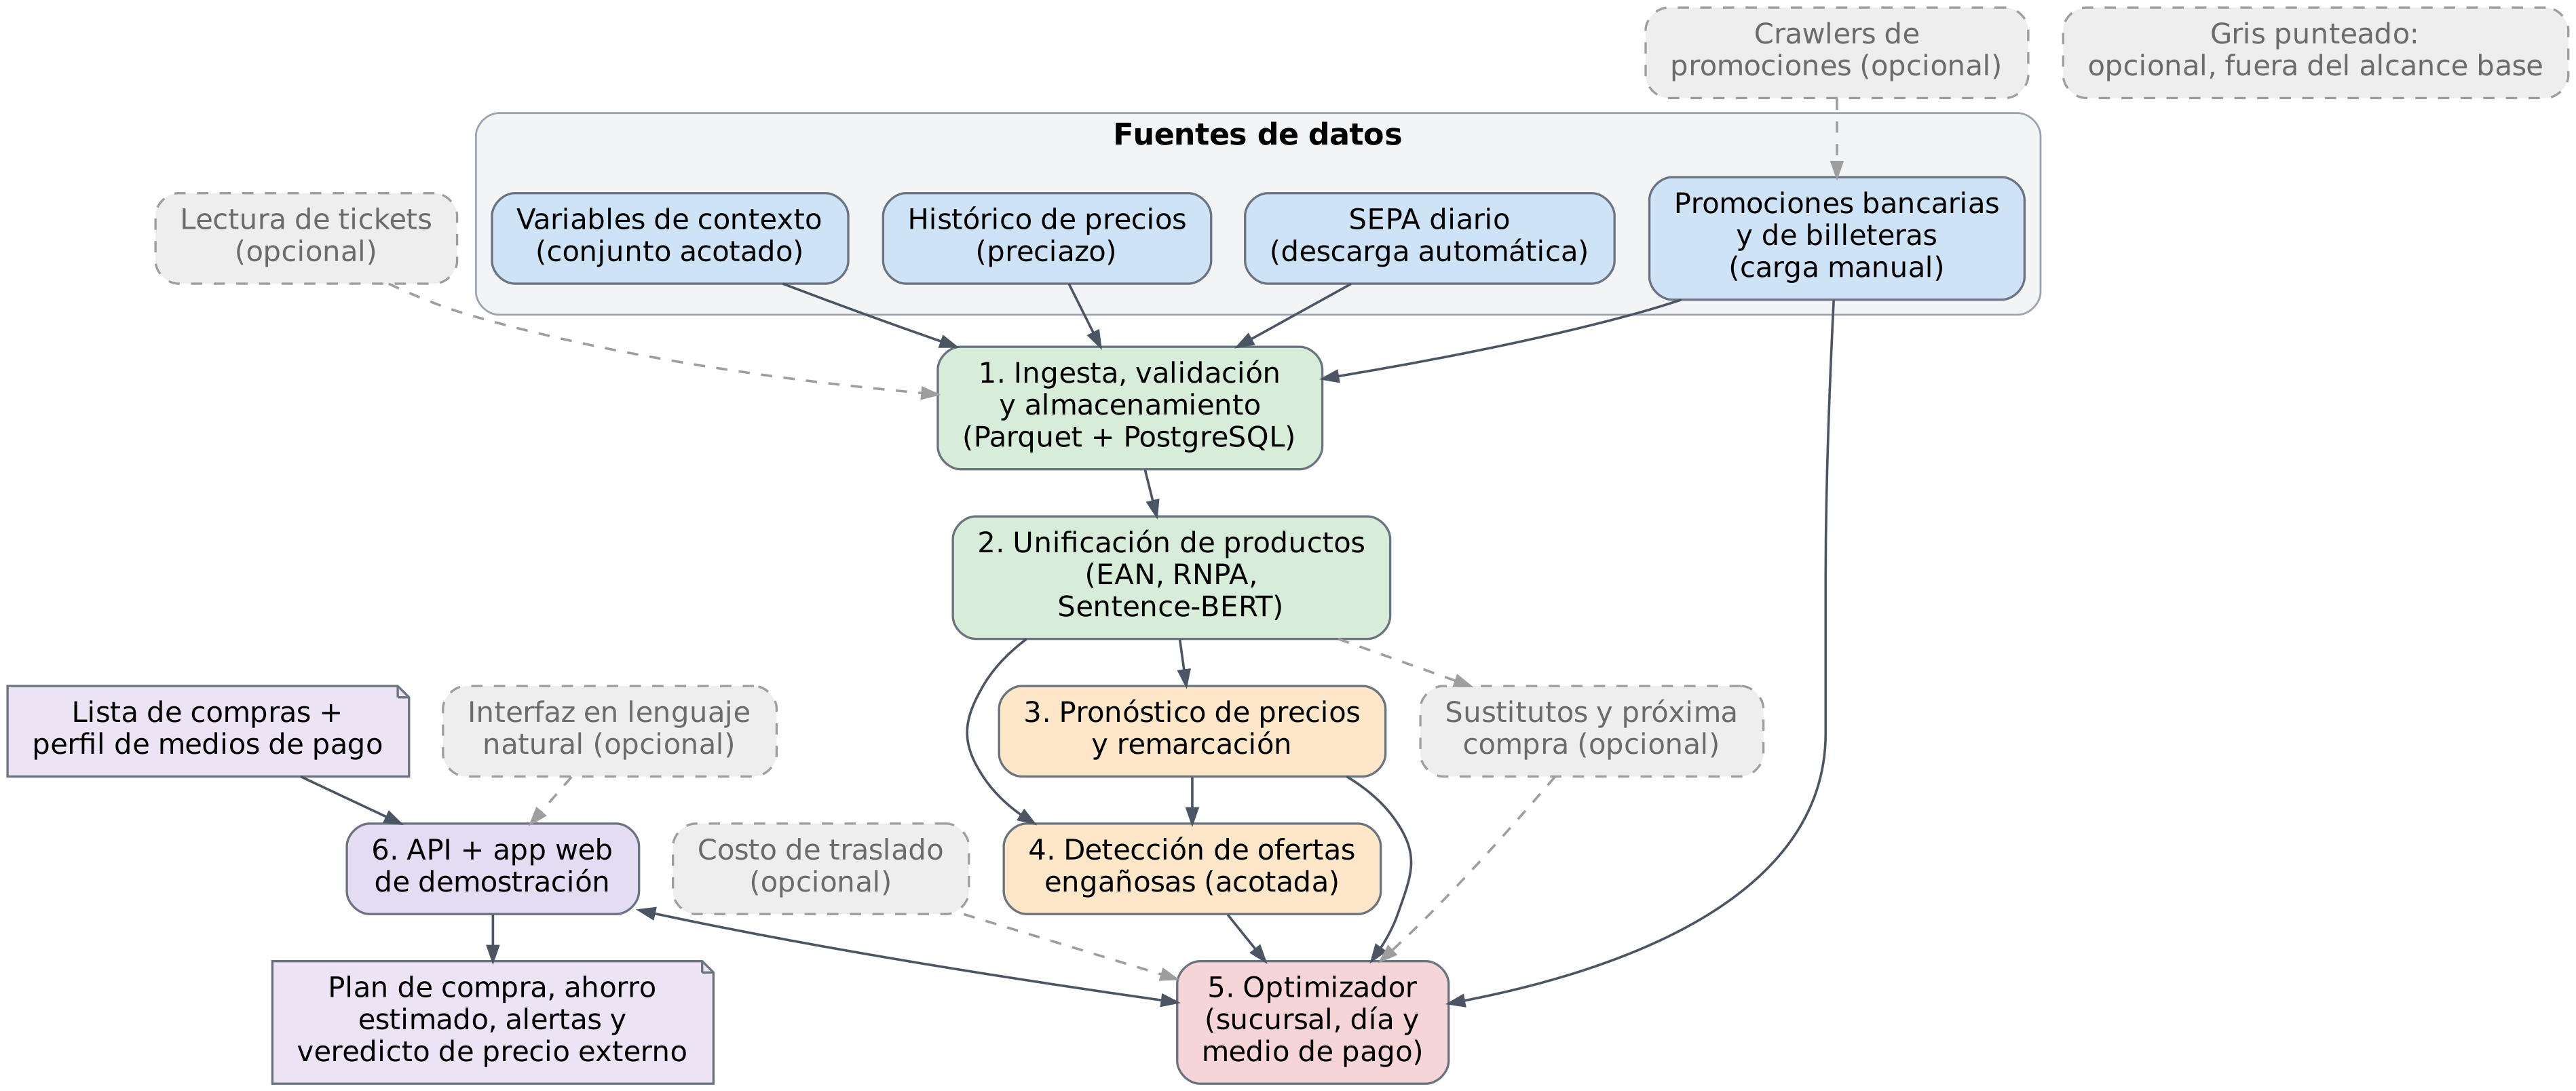
\includegraphics[width=\textwidth]{./Figuras/diagBloques-proyecto.png}
\caption{Diagrama en bloques del sistema propuesto.}
\label{fig:diagBloquesProyecto}
\end{figure}

La descripción funcional de cada bloque es la siguiente:

\begin{itemize}
	\item \textbf{Fuentes de datos:} archivos diarios de SEPA descargados de forma automática (en una máquina virtual en la nube, para no depender de la computadora personal), el histórico de precios de preciazo desde septiembre de 2024, las promociones bancarias y de billeteras cargadas manualmente (se publican en forma mensual) y un conjunto acotado de variables de contexto.
	\item \textbf{1. Ingesta, validación y almacenamiento:} limpieza, tratamiento de faltantes y detección de anomalías (por ejemplo, con Isolation Forest). Los datos se guardan en archivos Parquet y en una base PostgreSQL.
	\item \textbf{2. Unificación de productos:} identifica productos idénticos (por código EAN), del mismo elaborador (marcas propias, mediante el RNPA) y equivalentes (mediante \textit{embeddings} de Sentence-BERT y un clasificador de pares). La comparación se realiza siempre por kilogramo, litro o unidad.
	\item \textbf{3. Pronóstico de precios y remarcación:} estima cuándo y cuánto cambiará el precio de cada producto en cada sucursal, con intervalos de confianza.
	\item \textbf{4. Detección de ofertas engañosas (versión acotada):} identifica inflado previo del precio, precios anteriores inexistentes y descuentos menores a los anunciados.
	\item \textbf{5. Optimizador:} mediante programación entera mixta elige sucursal, día y medio de pago con menor costo esperado, respetando las promociones habilitadas por el perfil del usuario y sus topes.
	\item \textbf{6. API y aplicación web de demostración:} recibe la lista de compras, el perfil de medios de pago y las consultas de precios externos, y devuelve el plan de compra, el ahorro estimado, las alertas y el veredicto sobre precios externos (``conveniente'', ``similar'' o ``caro'').
\end{itemize}

\textbf{Ciclo de vida y cliente.} La solución se encuentra en etapa de concepto validado: se verificó la viabilidad técnica con archivos diarios de SEPA y se cuenta con el histórico necesario. El resultado del proyecto será un prototipo funcional evaluado, no un producto en producción. El adoptante de los entregables es el consumidor de supermercado sensible al precio, que dispone de varios medios de pago y valora un ahorro concreto, recomendaciones simples de seguir y poder confiar en que una oferta es real. El trabajo se centra en las cuatro cadenas principales de la ciudad de Paraná (Entre Ríos), que se toma como caso de uso real.

\textbf{Innovación.} La innovación pasa por integrar, sobre datos abiertos de Argentina, el pronóstico de precios, la detección de ofertas engañosas y la optimización bajo incertidumbre considerando el perfil de medios de pago del usuario, y por evaluar el sistema por el ahorro real en pesos que produce.

\section{2. Identificación y análisis de los interesados}
\label{sec:interesados}

\begin{table}[ht]
\caption{Identificación de los interesados.}
\label{tab:interesadosProyecto}
\begin{tabularx}{\linewidth}{@{}|l|X|X|X|@{}}
\hline
\rowcolor[HTML]{C0C0C0} 
Rol           & Nombre y Apellido & Organización 	& Puesto 	\\ \hline
Cliente       & \clientename      &\empclientename	& Director del Trabajo Final \\ \hline
Impulsor      & Federico G. Zacchigna & FIUBA        & Coordinación académica de IA \\ \hline
Responsable   & \authorname       & FIUBA        	& Alumno 	\\ \hline
Opositores    & -                 & Cadenas de supermercados alcanzadas & - \\ \hline
Usuario final & Consumidores de supermercados & - & - \\ \hline
\end{tabularx}
\end{table}

\begin{itemize}
	\item Cliente: el \clientename\hspace{1px} es docente de la CEIA en las asignaturas de Introducción a la Inteligencia Artificial, Aprendizaje de Máquina y Operaciones de Aprendizaje Automático. Valida el plan de trabajo y orienta en las decisiones de modelado y de despliegue. Acordó recibir un correo mensual con el estado de avance y responder consultas puntuales.
	\item Impulsor: Federico G. Zacchigna aprobó la propuesta de trabajo y sugirió incorporar la consulta de precios ofrecidos fuera de las cadenas principales.
	\item Responsable: el autor trabaja como ingeniero de software y desarrolla el proyecto en forma individual, por lo que la disponibilidad horaria debe compatibilizarse con su actividad laboral y con la cursada.
	\item Opositores: las cadenas de supermercados podrían objetar la publicación de análisis sobre ofertas engañosas. Se utilizan únicamente datos que las propias cadenas informan al SEPA y criterios explícitos y reproducibles.
	\item Usuario final: personas que compran en supermercados y disponen de distintos medios de pago. Para las pruebas se toma como caso de uso real la ciudad de Paraná.
\end{itemize}

\section{3. Propósito del proyecto}
\label{sec:proposito}

El propósito de este proyecto es ayudar a los consumidores a pagar menos por su compra de supermercado, recomendándoles dónde, cuándo y con qué medio de pago comprar, y protegiéndolos de ofertas engañosas. Para ello se busca desarrollar y evaluar un sistema basado en aprendizaje automático que aproveche los datos abiertos de precios de Argentina y cuyo valor pueda medirse como ahorro en pesos frente a la forma habitual de comprar.

\section{4. Alcance del proyecto}
\label{sec:alcance}

El alcance se ajustó respecto de la propuesta aprobada por la coordinación académica, por recomendación del director, para concentrarse en un núcleo que pueda completarse y evaluarse adecuadamente en 600 horas. Las funcionalidades que quedan fuera del núcleo se listan más abajo como opcionales y, si no llegan a abordarse, quedarán como trabajo futuro.

El proyecto incluye:

\begin{itemize}
	\item Descarga diaria automatizada de los archivos de SEPA y su almacenamiento histórico, junto con la incorporación del histórico de preciazo.
	\item Ingesta, limpieza y validación de los datos, con detección de anomalías.
	\item Las sucursales de las cuatro cadenas principales de Paraná: Coto, Carrefour, ChangoMás (incluido HiperChangoMás) y DIA. El \textit{pipeline} se diseñará de forma genérica para facilitar la incorporación posterior de otras sucursales o cadenas.
	\item Unificación de productos con código de barras:
		\begin{itemize}
		\item Productos idénticos por código EAN.
		\item Productos del mismo elaborador (marcas propias) mediante el RNPA.
		\item Productos equivalentes mediante Sentence-BERT y un clasificador de pares.
		\item Normalización del precio por kilogramo, litro o unidad.
		\end{itemize}
	\item Carga manual estructurada, con frecuencia mensual, de las promociones de las billeteras virtuales y los bancos con más promociones en esas cadenas, y de descuentos generales como los destinados a jubilados.
	\item Modelos de pronóstico de precios y de remarcación con intervalos de confianza, comparados contra modelos de referencia (\textit{baselines}), usando un conjunto acotado de variables de contexto.
	\item Una versión acotada de la detección de ofertas engañosas, basada en criterios explícitos (inflado previo del precio, precio anterior inexistente y descuento menor al anunciado).
	\item Optimizador que recomiende sucursal, día y medio de pago para una lista de compras y un perfil de medios de pago.
	\item Consulta de conveniencia de un precio ofrecido fuera de las cadenas principales (por ejemplo, en un almacén), frente a los datos disponibles.
	\item API y aplicación web simple de demostración.
	\item Evaluación del sistema mediante \textit{backtest} sobre compras simuladas, con partición temporal (entrenamiento de septiembre de 2024 a marzo de 2026 y prueba de julio a septiembre de 2026), con el ahorro en pesos frente a una estrategia ingenua como métrica central y métricas específicas por módulo.
	\item Documentación del código, memoria del trabajo final y defensa pública.
\end{itemize}

Funcionalidades opcionales, que se incorporarán solo si el cronograma lo permite, en orden de menor a mayor complejidad:

\begin{itemize}
	\item Incorporación de otras sucursales o cadenas, además de las cuatro mencionadas en Paraná.
	\item Incorporación de más variables macroeconómicas externas a los modelos de pronóstico.
	\item Interfaz en lenguaje natural basada en un modelo de lenguaje.
	\item \textit{Crawlers} para automatizar la carga de promociones bancarias y de billeteras.
	\item Caso de estudio de ofertas engañosas en electrodomésticos vendidos por las mismas cadenas en CyberMonday y Black Friday.
	\item Recomendación de productos sustitutos y predicción de la próxima compra.
	\item Cálculo de la distancia del usuario a cada sucursal para considerar el costo de traslado.
	\item Lectura y verificación de tickets de compra fotografiados, incluida la construcción del dataset correspondiente.
\end{itemize}

El presente proyecto no incluye:

\begin{itemize}
	\item La puesta en producción de la aplicación ni su publicación para usuarios externos.
	\item Productos sin código de barras (frescos) ni fotografías de góndolas o carteles de precios.
	\item Cadenas o comercios que no informan al SEPA, salvo como precio externo consultado por el usuario.
	\item Comercios de electrodomésticos o plataformas de comercio electrónico ajenas a las cadenas alcanzadas.
\end{itemize}

\section{5. Supuestos del proyecto}
\label{sec:supuestos}

Para el desarrollo del presente proyecto se supone que:

\begin{itemize}
	\item El SEPA continuará publicando a diario los precios de las cadenas alcanzadas, con un formato similar al actual, y la normativa que obliga a las cadenas a informarlos seguirá vigente.
	\item La descarga diaria automatizada funcionará sin interrupciones prolongadas y, ante fallas puntuales, el histórico de preciazo permitirá completar los faltantes.
	\item Los precios informados al SEPA representan con razonable fidelidad los precios en góndola de las sucursales.
	\item Las promociones bancarias y de billeteras seguirán publicándose en forma mensual y podrán cargarse manualmente en un tiempo acotado, sin necesidad de \textit{crawlers}.
	\item El autor dispondrá de aproximadamente 600 horas de trabajo entre octubre de 2026 y agosto de 2027, compatibles con su actividad laboral y con la cursada.
	\item Serán suficientes los recursos de cómputo disponibles: una computadora personal y una máquina virtual de la capa gratuita de Oracle Cloud, junto con herramientas y modelos preentrenados de código abierto.
	\item El director del trabajo estará disponible para responder consultas y recibir los informes mensuales de avance.
	\item El contexto macroeconómico mantendrá la variabilidad de precios y la diversidad de promociones que hacen relevante el problema; en caso de cambios significativos, la metodología seguirá siendo aplicable.
\end{itemize}

\section{6. Product Backlog}
\label{sec:backlog}

El Product Backlog debe organizarse en cuatro \textbf{\textit{\'{e}picas}} fundamentales del proyecto. Cada \'{e}pica debe contener al menos dos historias de usuario que describan funcionalidades clave.

El Product Backlog debe permitir interpretar cómo será el proyecto y su funcionalidad. Se deben indicar claramente las prioridades entre las historias de usuario y si hay alguna opcional.

Las historias de usuario deben ser breves, claras y medibles, expresando el rol, la necesidad y el propósito de cada funcionalidad. También deben tener una prioridad definida para facilitar la planificación de los sprints.

Cada historia de usuario debe incluir una ponderación en \textit{Story Points}, un número entero que representa el tama\~no relativo de la historia. El criterio para calcular los Story Points debe indicarse explícitamente.

Las historias deben seguir el formato: ``\textit{Como [rol], quiero [tal cosa] para [tal otra cosa]}''.

Las \'{e}picas deben estructurarse de la siguiente forma:

\begin{itemize}
  \item \textbf{\'{E}pica 1}
    \begin{itemize}
      \item HU1
      \item HU2
    \end{itemize}
  \item \textbf{\'{E}pica 2}
    \begin{itemize}
      \item HU3
      \item HU4
    \end{itemize}
  \item \textbf{\'{E}pica 3}
    \begin{itemize}
      \item HU5
      \item HU6
    \end{itemize}
  \item \textbf{\'{E}pica 4}
    \begin{itemize}
      \item HU7
      \item HU8
    \end{itemize}
\end{itemize}

\textbf{Reglas para definir historias de usuario:}
\begin{itemize}
  \item Ser concisas y claras.
  \item Expresarlas en términos cuantificables y medibles.
  \item No dejar margen para interpretaciones ambiguas.
  \item Indicar claramente su prioridad y si son opcionales.
  \item Considerar regulaciones y normas vigentes.
\end{itemize}

\section{7. Criterios de aceptación de historias de usuario}
\label{sec:criteriosAceptacion}

Los criterios de aceptación deben establecerse para cada historia de usuario, asegurando que se cumplan las condiciones necesarias para que la funcionalidad sea validada correctamente.

Cada historia debe tener criterios medibles, específicos y verificables. Deben permitir validar que se cumple con las necesidades del usuario.

Se estructuran de forma análoga a las \'{e}picas del backlog:

\begin{itemize}
  \item \textbf{\'{E}pica 1}
    \begin{itemize}
      \item Criterios de aceptación HU1
      \item Criterios de aceptación HU2
    \end{itemize}
  \item \textbf{\'{E}pica 2}
    \begin{itemize}
      \item Criterios de aceptación HU3
      \item Criterios de aceptación HU4
    \end{itemize}
  \item \textbf{\'{E}pica 3}
    \begin{itemize}
      \item Criterios de aceptación HU5
      \item Criterios de aceptación HU6
    \end{itemize}
  \item \textbf{\'{E}pica 4}
    \begin{itemize}
      \item Criterios de aceptación HU7
      \item Criterios de aceptación HU8
    \end{itemize}
\end{itemize}

\textbf{Reglas para definir criterios de aceptación:}
\begin{itemize}
  \item Medibles y verificables.
  \item Especificar cuándo una historia se considera completada.
  \item Incluir condiciones específicas.
  \item No ambiguos.
  \item Probables de testear funcional o técnicamente.
  \item Mínimo 3 criterios por HU.
\end{itemize}

\section{8. Fases de CRISP-DM}

\begin{enumerate}
  \item \textbf{Comprensión del negocio:} objetivo, valor agregado de IA, métricas de éxito.
  \item \textbf{Comprensión de los datos:} tipo, origen, cantidad, calidad.
  \item \textbf{Preparación de los datos:} características clave, transformaciones necesarias.
  \item \textbf{Modelado:} tipo de problema, algoritmos posibles.
  \item \textbf{Evaluación del modelo:} métricas de rendimiento.
  \item \textbf{Despliegue del modelo (opcional):} tipo de despliegue y herramientas.
\end{enumerate}

\section{9. Desglose del trabajo en tareas}
\label{sec:wbs}

A partir de cada Historia de Usuario (HU) definida en la sección 6, descomponer el trabajo en tareas técnicas concretas, medibles y acotadas en el tiempo.

\begin{itemize}
\item Seleccionar entre 2 y 3 tareas por cada historia de usuario.
\item Cada tarea debe estar claramente formulada, ser técnica, accionable y con una estimación horaria entre 2 y 8 horas.
\item Evitar tareas genéricas (como ''desarrollar funcionalidad´´) o demasiado amplias.
\item Si una tarea supera las 8 horas, debe dividirse en subtareas.
\item Indicar la prioridad relativa de cada tarea (Alta, Media o Baja).
\end{itemize}

\begin{table}[htpb]
\centering
\begin{tabularx}{\linewidth}{@{}|X|X|c|c|@{}}
\hline
\rowcolor[HTML]{C0C0C0}
Historia de usuario & Tarea técnica & Estimación & Prioridad \\ \hline
HU1 & Tarea 1 HU1 & 6 h & Alta \\ \hline
HU1 & Tarea 2 HU1 & 8 h & Alta \\ \hline
HU2 & Tarea 1 HU2 & 5 h & Media \\ \hline
HU2 & Tarea 2 HU2 & 6 h & Alta \\ \hline
... & ... & ... & ... \\ \hline
\end{tabularx}
\end{table}

\textbf{Criterios para estimar tiempos:}
\begin{itemize}
  \item Considerar la complejidad técnica, el nivel de incertidumbre y la experiencia previa.
  \item Evitar subestimar el esfuerzo: estimar el tiempo realista que llevaría implementar, testear y documentar cada tarea.
  \item Basar la estimación en la experiencia propia o en referencias de tareas similares.
\end{itemize}

\textbf{Sobre la prioridad:}
\begin{itemize}
  \item Asignar una prioridad relativa (Alta, Media o Baja) según la relevancia funcional de la tarea y su impacto en los entregables.
  \item Priorizar tareas que estén vinculadas a criterios de aceptación de las HU o que sean necesarias para desbloquear otras.
  \item Incluir tareas opcionales solo si están bien justificadas.
\end{itemize}

\textbf{Recomendaciones generales:}
\begin{itemize}
  \item -Enfocarse en tareas que surgen directamente de las HU planteadas.
  \item No es necesario cubrir las 600 horas del proyecto en esta sección: el foco está en el desglose de funcionalidades clave.
  \item Este trabajo será la base para organizar algunos de los sprints y elaborar el cronograma del proyecto, por lo que debe ser claro y realista.
\end{itemize}

\section{10. Planificación de Sprints}

Organizar las tareas técnicas del proyecto en sprints de trabajo que permitan distribuir de forma equilibrada la carga horaria total, estimada en 600 horas.

\textbf{Consigna:}
\begin{itemize}
  \item Completar una tabla que relacione sprints con HU y tareas técnicas correspondientes.
  \item Incluir estimación en horas para cada tarea.
  \item Indicar responsable y porcentaje de avance estimado o completado.
  \item Contemplar también tareas de planificación, documentación, redacción de memoria y preparación de defensa.
\end{itemize}

\textbf{Conceptos clave:}
\begin{itemize}
  \item Una \'{e}pica es una unidad funcional amplia; una historia de usuario es una funcionalidad concreta; un sprint es una unidad de tiempo donde se ejecutan tareas.
  \item Las tareas son el nivel más desagregado: permiten estimar tiempos, asignar responsables y monitorear progreso.
\end{itemize}

\textbf{Duración sugerida:}
\begin{itemize}
  \item Para un proyecto de 600 h, se recomienda planificar entre 10 y 12 sprints de aproximadamente 2 semanas cada uno.
  \item Asignar entre 45 y 50 horas efectivas por sprint a tareas técnicas.
  \item Reservar 100 a 120 h para actividades no técnicas (planificación, escritura, reuniones, defensa).
\end{itemize}

\textbf{Importante:}
\begin{itemize}
  \item En proyectos individuales, el responsable suele ser el propio autor.
  \item Aun así, desagregar tareas facilita el seguimiento y mejora continua.
\end{itemize}

\textbf{Conversión opcional de Story Points a horas:}
\begin{itemize}
  \item 1 SP \(\approx\) 2 h como referencia flexible.
  \item Tener en cuenta aproximaciones tipo Fibonacci.
\end{itemize}

\begin{table}[htpb]
\centering
\caption{Formato sugerido}
\begin{tabularx}{\linewidth}{@{}|l|l|X|c|l|c|@{}}
\hline
\rowcolor[HTML]{C0C0C0}
Sprint & HU o fase & Tarea & Horas / SP & Responsable & \% Completado \\ \hline
Sprint 0 & Planificación & Definir alcance y cronograma & 10 h & Alumno & 100\% \\ \hline
Sprint 0 & Planificación & Reunión con el tutor/cliente & 5 h & Alumno & 50\% \\ \hline
Sprint 0 & Planificación & Ajuste de los entregables & 6 h & Alumno & 25\% \\ \hline
Sprint 1 & HU1 & Tarea 1 HU1 & 6 h / 3 SP & Alumno & 0\% \\ \hline
Sprint 1 & HU1 & Tarea 2 HU1 & 10 h / 5 SP & Alumno & 0\% \\ \hline
Sprint 2 & HU2 & Tarea 1 HU2 & 7 h / 5 SP & Alumno & 0\% \\ \hline
... & ... & ... & ... & ... & ... \\ \hline
Sprint 5 & Escritura & Redacción memoria & 50 h / 34 SP & Alumno & 0\% \\ \hline
Sprint 6 & Defensa & Preparación de la exposición & 20 h / 13 SP & Alumno & 0\% \\ \hline
\end{tabularx}
\end{table}

\textbf{Recomendaciones:}
\begin{itemize}
  \item Verificar que la carga horaria por sprint sea equilibrada.
  \item Usar sprints de 1 a 3 semanas, acordes al cronograma general.
  \item Actualizar el \% completado durante el seguimiento del proyecto.
  \item Considerar un sprint final exclusivo para pruebas, revisión y ajustes antes de la defensa.
\end{itemize}


\section{11. Diagrama de Gantt (sprints)}
\label{sec:gantt}

Visualizar en un diagrama de Gantt la planificación temporal del proyecto, tomando como base los sprints definidos en la sección anterior. Debe contemplar todas las horas del proyecto.

Consigna:

\begin{itemize}

\item Elaborar un diagrama de Gantt que muestre la secuencia temporal de los sprints.

\item Cada fila debe representar un sprint (con su número o nombre), y el eje horizontal debe indicar el tiempo (en semanas o fechas concretas).

\item Las tareas técnicas derivadas de HU deben diferenciarse visualmente (por ejemplo, con un color distinto) de las tareas no técnicas (planificación, redacción, defensa).

\item Incluir todas las tareas estimadas en cada sprint.
\end{itemize}

Recomendaciones para el Gantt:

\begin{itemize}

	\item Podés usar herramientas gratuitas como TeamGantt, ClickUp, GanttProject, [Google Sheets], [Trello + Planyway], entre otras.
	\item Ordená los sprints de forma cronológica, comenzando con Sprint 0 (planificación) y finalizando con el sprint de defensa.
	\item Asegurate de reflejar la duración realista de cada sprint según tu disponibilidad y el cronograma general del posgrado.
	\item Incluí hitos importantes: reuniones, entregas parciales, defensa.
\end{itemize}


Incluir una imagen legible del diagrama de Gantt. Si es muy ancho, presentar primero la tabla y luego el gráfico de barras.



\section{12. Gobernanza de datos}
\label{sec:gobernanza}

En esta sección se debe analizar de manera integral el marco normativo y ético asociado al uso de los datos y al desarrollo de soluciones basadas en inteligencia artificial.

El análisis se divide en dos partes:

\begin{itemize}
  \item Cumplimiento normativo.
  \item Ética en el uso de inteligencia artificial.
\end{itemize}

\subsection{Cumplimiento normativo}
Este análisis es clave para garantizar el cumplimiento normativo y evitar conflictos legales durante el desarrollo y publicación del proyecto.

En esta subsección se debe identificar si los datos utilizados en el proyecto están sujetos a normativas de protección de datos y privacidad, y en qué condiciones pueden emplearse.

Aspectos a considerar:

\begin{itemize}
  \item Determinar si los datos están regulados por normativas como el GDPR, la Ley 25.326 de Protección de Datos Personales (Argentina), la HIPAA u otras, según la jurisdicción o la temática del proyecto.
  \item Aclarar si las fuentes de datos son propias, de acceso público o licenciadas. En este último caso, explicitar la licencia correspondiente y sus condiciones de uso. Realizar este mismo análisis para las herramientas y, en caso de corresponder, para los modelos preentrenados a emplear.
  \item Analizar la viabilidad legal del proyecto, considerando los mecanismos necesarios para garantizar el cumplimiento normativo y la trazabilidad de los datos.
\end{itemize}

\subsection{Ética en el uso de inteligencia artificial}

En esta subsección se debe reflexionar sobre los aspectos éticos vinculados al uso de datos y algoritmos de inteligencia artificial. Se espera una evaluación de la integridad del sistema y su impacto social.

Aspectos a considerar:

\begin{itemize}
	\item Identificar posibles sesgos en los datos o modelos (ideológicos, culturales, de género, geográficos, etc.) y analizar sus consecuencias (por ejemplo: discriminación, manipulación, pérdida de privacidad o desinformación).
	\item Analizar los posibles riesgos en términos de impacto social del uso indebido de la solución a desarrollar.
	\item En caso de corresponder, proponer medidas de mitigación y mecanismos de confianza (auditorías, documentación, trazabilidad, revisión humana, etc.).
	\item Finalmente, elaborar una reflexión general sobre la ética del proyecto, considerando tanto la equidad y transparencia del sistema como su impacto potencial en la sociedad.

\end{itemize}


\section{13. Gestión de riesgos}
\label{sec:riesgos}

\begin{consigna}{red}
a) Identificación de los riesgos (al menos cinco) y estimación de sus consecuencias:
 
Riesgo 1: detallar el riesgo (riesgo es algo que si ocurre altera los planes previstos de forma negativa)
\begin{itemize}
	\item Severidad (S): mientras más severo, más alto es el número (usar números del 1 al 10).\\
	Justificar el motivo por el cual se asigna determinado número de severidad (S).
	\item Probabilidad de ocurrencia (O): mientras más probable, más alto es el número (usar del 1 al 10).\\
	Justificar el motivo por el cual se asigna determinado número de (O). 
\end{itemize}   

Riesgo 2:
\begin{itemize}
	\item Severidad (S): X.\\
	Justificación...
	\item Ocurrencia (O): Y.\\
	Justificación...
\end{itemize}

Riesgo 3:
\begin{itemize}
	\item Severidad (S):  X.\\
	Justificación...
	\item Ocurrencia (O): Y.\\
	Justificación...
\end{itemize}


b) Tabla de gestión de riesgos:      (El RPN se calcula como RPN=SxO)

\begin{table}[htpb]
\centering
\begin{tabularx}{\linewidth}{@{}|X|c|c|c|c|c|c|@{}}
\hline
\rowcolor[HTML]{C0C0C0} 
Riesgo & S & O & RPN & S* & O* & RPN* \\ \hline
       &   &   &     &    &    &      \\ \hline
       &   &   &     &    &    &      \\ \hline
       &   &   &     &    &    &      \\ \hline
       &   &   &     &    &    &      \\ \hline
       &   &   &     &    &    &      \\ \hline
\end{tabularx}%
\end{table}

Criterio adoptado: 

Se tomarán medidas de mitigación en los riesgos cuyos números de RPN sean mayores a...

Nota: los valores marcados con (*) en la tabla corresponden luego de haber aplicado la mitigación.

c) Plan de mitigación de los riesgos que originalmente excedían el RPN máximo establecido:
 
Riesgo 1: plan de mitigación (si por el RPN fuera necesario elaborar un plan de mitigación).
  Nueva asignación de S y O, con su respectiva justificación:
  \begin{itemize}
	\item Severidad (S*): mientras más severo, más alto es el número (usar números del 1 al 10).
          Justificar el motivo por el cual se asigna determinado número de severidad (S).
	\item Probabilidad de ocurrencia (O*): mientras más probable, más alto es el número (usar del 1 al 10).
          Justificar el motivo por el cual se asigna determinado número de (O).
	\end{itemize}

Riesgo 2: plan de mitigación (si por el RPN fuera necesario elaborar un plan de mitigación).
 
Riesgo 3: plan de mitigación (si por el RPN fuera necesario elaborar un plan de mitigación).

\end{consigna}

\section{14. Sprint Review}
\label{sec:sprint_review}

La revisión de sprint (\emph{Sprint Review}) es una práctica fundamental en metodologías ágiles. Consiste en revisar y evaluar lo que se ha completado al finalizar un sprint. En esta instancia, se presentan los avances y se verifica si las funcionalidades cumplen con los criterios de aceptación establecidos. También se identifican entregables parciales y se consideran ajustes si es necesario.

Aunque el proyecto aún se encuentre en etapa de planificación, esta sección permite proyectar cómo se evaluarán las funcionalidades más importantes del backlog. Esta mirada anticipada favorece la planificación enfocada en valor y permite reflexionar sobre posibles obstáculos.

\textbf{Objetivo:} anticipar cómo se evaluará el avance del proyecto a medida que se desarrollen las funcionalidades, utilizando como base al menos cuatro historias de usuario del \emph{Product Backlog}.


Seleccionar al menos 4 HU del Product Backlog. Para cada una, completar la siguiente tabla de revisión proyectada:

\textbf{Formato sugerido:}
\begin{table}[htpb]
\renewcommand{\arraystretch}{1.5}
\begin{tabular}{|>{\raggedright\arraybackslash}m{2.4cm}|
                >{\raggedright\arraybackslash}m{2.3cm}|
                >{\raggedright\arraybackslash}m{3cm}|
                >{\raggedright\arraybackslash}m{3cm}|
                >{\raggedright\arraybackslash}m{3cm}|}
\hline
\rowcolor[HTML]{CCCCCC}
\textbf{HU seleccionada} & \textbf{Tareas asociadas} & \textbf{Entregable esperado} & \textbf{¿Cómo sabrás que está cumplida?} & \textbf{Observaciones o riesgos} \\
\hline
                         & Tarea 1 &                             &                                           &                                     \\ \cline{2-2}
\multirow{-2}{=}{HU1}    & Tarea 2 & \multirow{-2}{=}{Módulo funcional} & \multirow{-2}{=}{Cumple criterios de aceptación definidos} & \multirow{-2}{=}{Falta validar con el tutor} \\
\hline
                         & Tarea 1 &                             &                                           &                                     \\ \cline{2-2}
\multirow{-2}{=}{HU3}    & Tarea 2 & \multirow{-2}{=}{Reporte generado} & \multirow{-2}{=}{Exportación disponible y clara} & \multirow{-2}{=}{Requiere datos reales} \\
\hline
                         & Tarea 1 &                             &                                           &                                     \\ \cline{2-2}
\multirow{-2}{=}{HU5}    & Tarea 2 & \multirow{-2}{=}{Panel de gestión} & \multirow{-2}{=}{Roles diferenciados operativos} & \multirow{-2}{=}{Riesgo en integración} \\
\hline
                         & Tarea 1 &                             &                                           &                                     \\ \cline{2-2}
\multirow{-2}{=}{HU7}    & Tarea 2 & \multirow{-2}{=}{Informe trimestral} & \multirow{-2}{=}{PDF con gráficos y evolución} & \multirow{-2}{=}{Puede faltar tiempo para ajustes} \\
\hline
\end{tabular}
\end{table}

\section{15. Sprint Retrospective}    
\label{sec:sprint_retro}

La retrospectiva de sprint es una práctica orientada a la mejora continua. Al finalizar un sprint, el equipo (o el alumno, si trabaja de forma individual) reflexiona sobre lo que funcionó bien, lo que puede mejorarse y qué acciones concretas pueden implementarse para trabajar mejor en el futuro.

Durante la cursada se propuso el uso de la \textbf{Estrella de la Retrospectiva}, que organiza la reflexión en torno a cinco ejes:

\begin{itemize}
\item  ¿Qué hacer más?
\item  ¿Qué hacer menos?
\item  ¿Qué mantener?
\item  ¿Qué empezar a hacer?
\item  ¿Qué dejar de hacer?
\end{itemize}

Aun en una etapa temprana, esta herramienta permite que el alumno planifique su forma de trabajar, identifique anticipadamente posibles dificultades y diseñe estrategias de organización personal.

\textbf{Objetivo:} reflexionar sobre las condiciones iniciales del proyecto, identificando fortalezas, posibles dificultades y estrategias de mejora, incluso antes del inicio del desarrollo.


Completar la siguiente tabla tomando como referencia los cinco ejes de la Estrella de la Retrospectiva (\emph{Starfish} o estrella de mar). Esta instancia te ayudará a definir buenas prácticas desde el inicio y prepararte para enfrentar el trabajo de forma organizada y flexible. Se deberá completar la tabla al menos para 3 sprints técnicos y 1 no técnico.

\textbf{Formato sugerido:}

\begin{table}[htpb]
\renewcommand{\arraystretch}{1.4}
\begin{tabular}{|>{\raggedright\arraybackslash}p{1.8cm}|
                >{\raggedright\arraybackslash}p{2.3cm}|
                >{\raggedright\arraybackslash}p{2.3cm}|
                >{\raggedright\arraybackslash}p{2.3cm}|
                >{\raggedright\arraybackslash}p{2.3cm}|
                >{\raggedright\arraybackslash}p{2.3cm}|}
\hline
\rowcolor[HTML]{CCCCCC} 
\textbf{Sprint tipo y N°} & \textbf{¿Qué hacer más?} & \textbf{¿Qué hacer menos?} & \textbf{¿Qué mantener?} & \textbf{¿Qué empezar a hacer?} & \textbf{¿Qué dejar de hacer?} \\
\hline
Sprint técnico - 1 & Validaciones continuas con el alumno & Cambios sin versión registrada & Pruebas con datos simulados & Documentar cambios propuestos & Ajustes sin análisis de impacto \\
\hline
Sprint técnico - 2 & Verificar configuraciones en múltiples escenarios & Modificar parámetros sin guardar historial & Perfiles reutilizables & Usar logs para configuración & Repetir pruebas manuales innecesarias \\
\hline
Sprint técnico - 8 & Comparar correlaciones con casos previos & Cambiar parámetros sin justificar & Revisión cruzada de métricas & Anotar configuraciones usadas & Trabajar sin respaldo de datos \\
\hline
Sprint no técnico - 12 (por ej.: ``Defensa'') & Ensayos orales con feedback & Cambiar contenidos en la memoria & Material visual claro & Dividir la presentación por bloques & Agregar gráficos difíciles de explicar \\
\hline
\end{tabular}
\end{table}




\end{document}